\documentclass[a4paper,11pt]{article}

\usepackage{amsmath}
\usepackage{array}
\usepackage{booktabs}
\usepackage{enumitem}
\usepackage{float}
\usepackage{float}
\usepackage{geometry}
\usepackage{graphicx}
\usepackage[labelfont=bf,font=footnotesize]{caption}
\usepackage{microtype}
\usepackage{parskip}
\usepackage{setspace}
\usepackage{siunitx}
\usepackage{subcaption}
\usepackage{titlesec}
\usepackage{xcolor}
\usepackage{xfrac}

\usepackage[hypertexnames=false,hidelinks]{hyperref}
\usepackage[noabbrev,nameinlink,capitalize,poorman]{cleveref}

% \captionsetup{font=footnotesize}
\bibliographystyle{unsrt}

\newcommand{\tpdf}[1]{\texorpdfstring{#1}{}}

\begin{document}

\begin{titlepage}
	\centering
	\includegraphics[width=\textwidth]{City\_logo.jpg} \\[4em]
	\begin{bfseries}
		\begin{Huge}
			Deep Learning for Image Analysis \\[35pt]
			\textsl{Written Report}
		\end{Huge}
	\end{bfseries}
	\vfill{}
	\begin{LARGE}
		\begin{sffamily}
			Martin Fixman and Grigorios Vaitsas \\[10pt]
			2023/2024 Term
		\end{sffamily}
	\end{LARGE}
\end{titlepage}

\section{Introduction}
\subsection{Overview}

In this study we have attempted to harness the power of deep learning techniques in order to analyse and understand the content of an image. More specifically, our aim was to create a program that, provided with an image of an urban environment, will be able to accurately identify and classify the different elements that make up the scene. In computer vision literature this task is called image segmentation. In image segmentation (often also referred to as dense prediction) the goal is to break down an image at pixel level into areas (segments) that correspond to different classes of objects. In our case the type of these classes would correspond to elements usually found in the urban landscape, such as roads, buildings, persons, cars, trees etc. A tool that allows to perform this task could have several applications. For example, it could be used to enhance vehicle security by being able to promptly alert drivers when a pedestrian or bicycle is detected in the projected path of the car. It could also be useful in creating applications for vehicle autonomy, where a car is able to navigate its environment and trace a safe path ahead without the need human input. 

Semantic segmentation is typically performed using deep learning methods, particularly convolutional neural networks (CNNs) and their variants as well as more recent attention-based models. In this study we have deployed the freely available Cityscapes dataset \cite{DBLP:journals/corr/CordtsORREBFRS16} which is a state-of-the-art dataset used for this particular type of analysis. We have created and trained three different models, with distinct characteristics and architectures and have evaluated their performance. We have performed a parameter sweep analysis to find the set of values that gives us the best results. 



\subsection{Dataset}

The Cityscapes dataset is a large-scale dataset widely used for training, evaluating and benchmarking algorithms in the fields of computer vision, particularly for models used to perform semantic segmentation and instance segmentation of urban street scenes. It consists of high resolution images captured from a vehicle-mounted camera while driving through 50 different cities in Germany and neighbouring countries. The capturing apparatus was equipped with a dual lens camera for stereoscopic capability, allowing for the possibility of applying stereo vision techniques useful for tasks like depth estimation, 3D reconstruction and scene understanding. 

The images that are used in our analysis are located in the folder \textbf{leftImg8bit}. These, as the name suggests, are taken from the left lens of the stereo camera system. They form the main high-resolution images (2048$\times$1024 pixels) with an 8-bit color depth that are used for all semantic and instance segmentation tasks using this dataset. Each image is stored in a PNG file format with a size that varies between 2.0 and 2.5 MB. The images have an RGB color space, which means that there are 3 color channels for each image.

The dataset comes with two different types of image annotations:\\
\textbf{Fine annotations:} Figure \ref{fig:cityscapes}(b). These provide detailed, pixel-level annotations for 5,000 images which have labels for 30 classes such as road, car, pedestrian, building, and traffic light. This dataset is split into 2,975 annotations for training, 500 for validation and 1,525 for testing. It is worth mentioning that the ground truth annotations for the testing set are not available to the users in order to allow for fair evaluation and benchmarking of models. Users instead need to submit their code to an online evaluation server which provides the quantitative performance metrics.    

\textbf{Coarse annotations:} Figure \ref{fig:cityscapes}(a). These include a much larger set of 20,000 images with less precise annotations intended for data augmentation and for tasks where granularity is not critical. The coarse annotations are split into a training and validation set. No test set is provided since this is only done using the fine annotations set. 

\begin{figure}[ht]
    \centering
    \begin{subfigure}{0.45\textwidth}
        \centering
        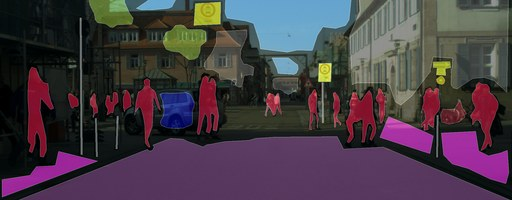
\includegraphics[width=\linewidth]{coarse_example.jpg}
        \caption{Coarse mask}
        \label{fig:sub1}
    \end{subfigure}\hfill
    \begin{subfigure}{0.45\textwidth}
        \centering
        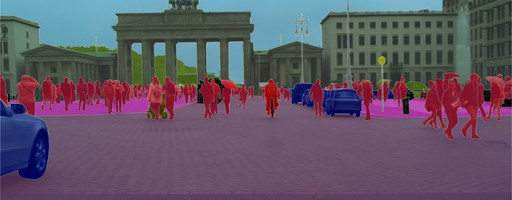
\includegraphics[width=\linewidth]{fine_example.jpg}
        \caption{Fine mask}
        \label{fig:sub2}
    \end{subfigure}
    \caption{Examples of coarse (a) and fine (b) mask annotations superimposed on the corresponding original images}
    \label{fig:cityscapes}
\end{figure}

The scenes in the CityScapes dataset represent a variety of urban settings, seasons, daylight conditions, and weather scenarios, providing robust, real-world environments for training models that need to perform under varied conditions. This dataset has been widely used in research for developing, testing and benchmarking new algorithms for computer vision tasks, gaining a place alongside datasets as iconic as ImageNet, COCO and Pascal VOC. The Cityscapes dataset can be accessed in the following address:
\begin{center}
\url{https://www.cityscapes-dataset.com}
\end{center}
Our particular approach in this study has been to start off by training a relatively simple model, that forms our baseline model, and then experiment with increasingly complex architectures. We aim to demonstrate that all these models are able to perform the task and further than that to investigate how the choice of various hyper-parameters and tweaks in architecture can affect the accuracy and performance of the models. The architectures that we have deployed in our study are briefly outlined in the section below.


\clearpage{}

\section{Architectures}
\subsection{Fully Convolutional Netowrk}

Modern, state-of-the-art techniques for image analysis involve convolutional neural networks (CNNs) in their implementation. CNNs can be used to extract vital information from spatial features, which allow us to classify and segment objects in images. A type of neural network architecture designed specifically for semantic segmentation is the Fully Convolutional Network (FCN). This architecture, developed by researchers from UC Berkeley in 2014 \cite{DBLP:journals/corr/LongSD14}, has been influential in advancing the field of computer vision, particularly in tasks requiring dense prediction, like semantic segmentation. 

\begin{figure}
    \centering 
    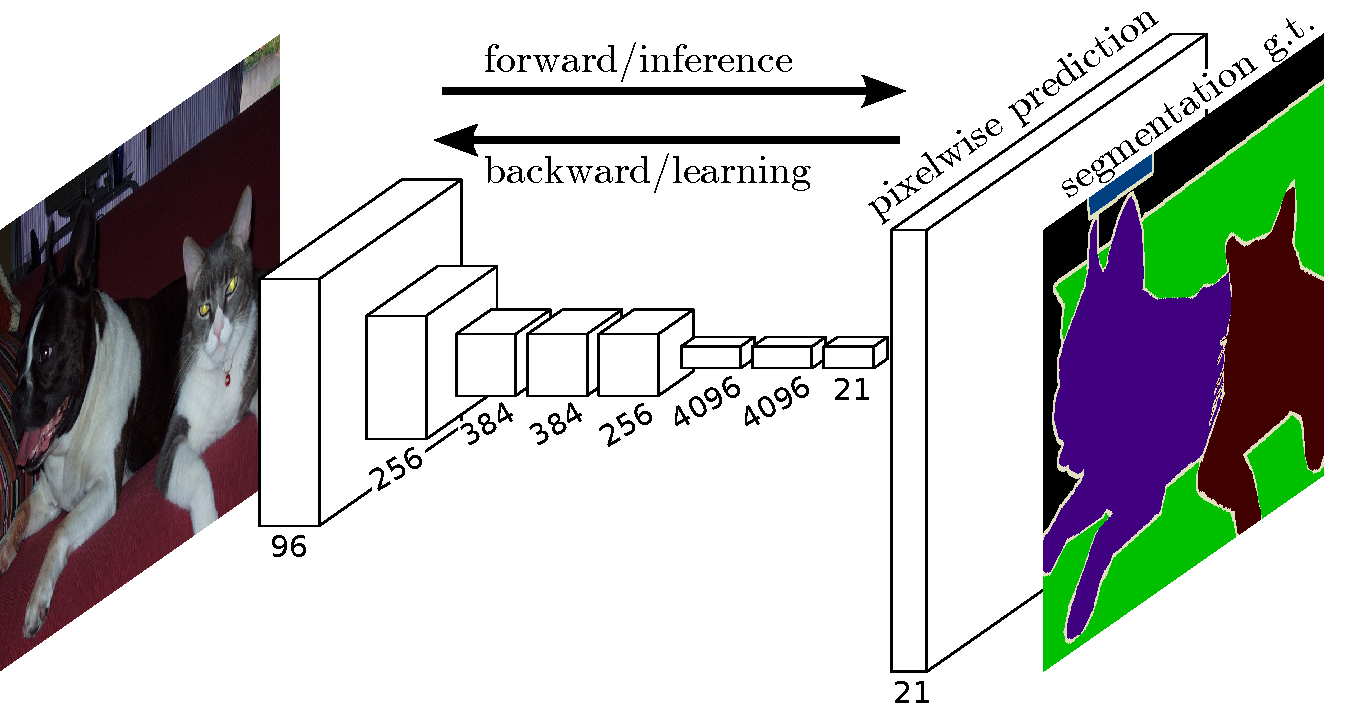
\includegraphics[width=0.7\textwidth]{alex-model.pdf}
    \caption{Example of a fully convolutional network used for semantic segmentation \cite{DBLP:journals/corr/LongSD14}}
    \label{fig:fcn-arch}
\end{figure}

Unlike standard convolutional neural networks used for image classification, which typically end with fully connected layers, FCNs are composed entirely of convolutional layers. This design allows them to take input of any size and output segmentation maps that correspond spatially to the input image, providing a per-pixel classification. FCNs transform the fully connected layers found in traditional CNNs (like those in AlexNet or VGGNet) into convolutional layers (Figure \ref{fig:fcn-arch}). This is done by treating the fully connected layers as convolutions with kernels that cover the entire input region. For example a fully connected layer that accepts an input of size 16$\times$16 can be reimagined as a convolutional layer with a 16$\times$16 filter size. To generate output segmentation maps that match the size of the input image, FCNs use transposed convolution layers (also known as deconvolutional layers) for upsampling. This process helps in recovering the spatial dimensions that are reduced during the pooling or convolutional operations in earlier layers. FCNs often utilize skip connections to combine deep, semantic information from lower layers with the shallow, appearance information in the upper layers of the network. This helps in improving the accuracy and detail of the output segmentation maps, as it allows the network to use both high-level and low-level features. 

\subsection{U-net}

Further improving upon the architecture of the fully convolutional network, the U-net, first introduced in a paper by Olaf Ronneberger, Philipp Fischer and Thomas Brox in 2015 \cite{DBLP:journals/corr/RonnebergerFB15}, has become very popular due to its efficiency and effectiveness, especially where data is limited. U-Net's architecture is distinctive because of its symmetric shape, which resembles the letter ``U'' (see Figure \ref{fig:u-netarch}). 
\begin{figure}
    \centering 
    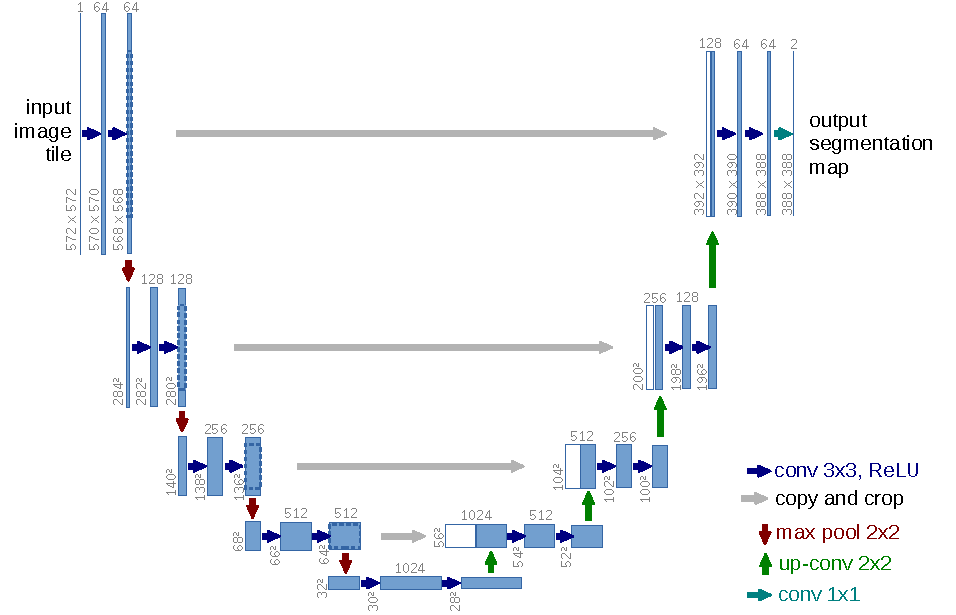
\includegraphics[width=0.7\textwidth]{u-net-illustration-correct-scale2.pdf}
    \caption{Example of the original U-net architecture as presented in \cite{DBLP:journals/corr/RonnebergerFB15}}
    \label{fig:u-netarch}
\end{figure}
It consists of two main parts: the left side of the U-net is the contracting path (encoder) which is designed to capture the context of the input image. This path is essentially a typical convolutional network that consists of repeated application of convolutions, followed by rectified linear unit (ReLU) activations, and max pooling for downsampling. Each of these steps helps in capturing the features at different levels of abstraction. On the right side of the network is the expansive path (Decoder), which performs the task of precise localization using transposed convolutions for upsampling. This part of the network gradually recovers the spatial dimensions and detail of the input image. The upsampling in the expansive path is combined with the high-resolution features from the contracting path via skip connections. These connections are crucial as they help in propagating context information to higher resolution layers, which enhances the accuracy of the output segmentation maps. U-Net's design is particularly effective in providing good segmentation results even with small training datasets, which has led to its widespread adoption and adaptation in different segmentation tasks beyond its initial medical imaging focus.

\subsection{Vision Transformer and Swin Transformer}

The last architecture we explored in our study was a Vision Transformer (ViT), which is a novel approach to applying transformer models, primarily used in Natural Language Processing (NLP) tasks, to image recognition. In the paper ``An Image is worth 16$\times$16 Words: Transformers for Image Recognition at scale'' \cite{DBLP:journals/corr/abs-2010-11929}, the authors proposed a method that treats an image as a sequence of fixed-size patches (similar to words in NLP). Each patch is embedded similarly to how tokens are embedded in NLP, and then processed by a standard transformer encoder. An overview of this model is depicted in Figure \ref{fig:vit-arch}.

\begin{figure}
    \centering 
    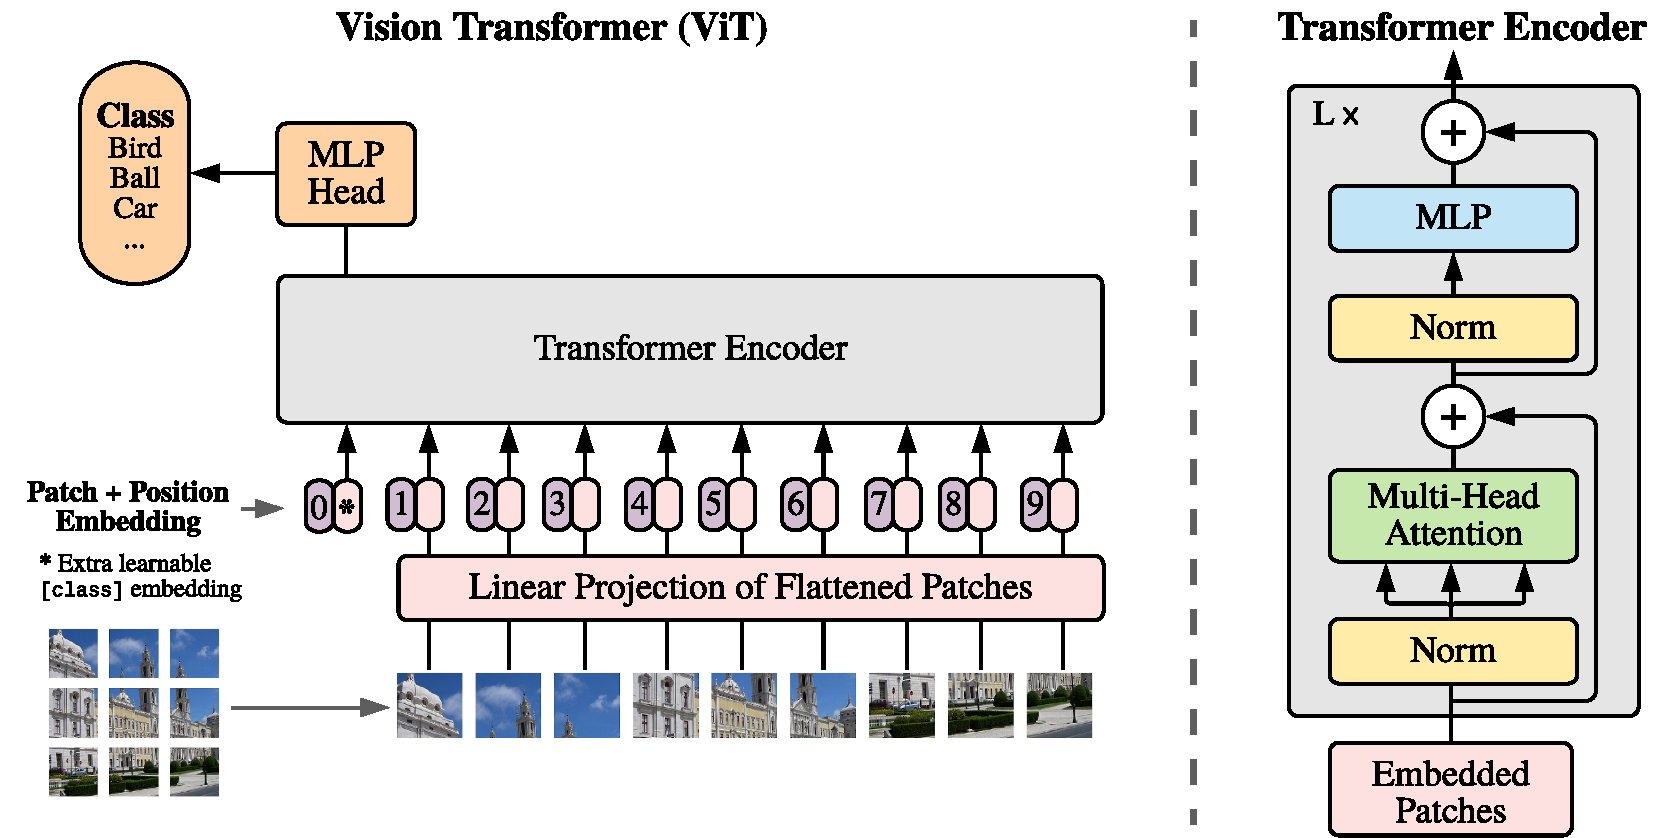
\includegraphics[width=0.8\textwidth]{model_scheme.pdf}
    \caption{Model overview of a Vision Transformer \cite{DBLP:journals/corr/RonnebergerFB15}}
    \label{fig:vit-arch}
\end{figure}

Vision transformers can achieve excellent results, outperforming many advanced CNN architectures, particularly when pre-trained on very large datasets. However, the computational complexity especially when applied on high-resolution images increases rapidly, especially for dense prediction tasks like semantic segmentation. For this reason, an improved approach has been suggested called the Swin Transformer model \cite{DBLP:journals/corr/abs-2103-14030}. In contrast to the Vision Transformer that processes the entire image at once by dividing it into fixed-size patches and applying global self-attention to all patches, the Swin transformer divides the image into smaller, non overlapping windows and applies local window-based self-attention (Figure \ref{fig:swintransform}(a)). This reduces the computational complexity because the number of interactions is limited to within a window rather than across the entire image. Additionally, the Swin transformer introduces a novel mechanism of shifting these windows in alternate layers, thus enabling cross-window connections. This helps in integrating local and global contextual information more effectively (Figure \ref{fig:swintransform}(b)). Finally, the fact that the Swin transformer starts with smaller windows and gradually merges them, reducing resolution while increasing the depth of features, enables a hierarchical architecture that processes features at multiple scales. This is beneficial for various vision tasks like object detection and segmentation, where multi-scale features are crucial. These advantages make the Swin transformer suitable as a general purpose backbone for various vision tasks and as will be explained later, we found this model to perform very well in our particular study.

\begin{figure}[ht]
    \centering
    \begin{subfigure}{0.45\textwidth}
        \centering
        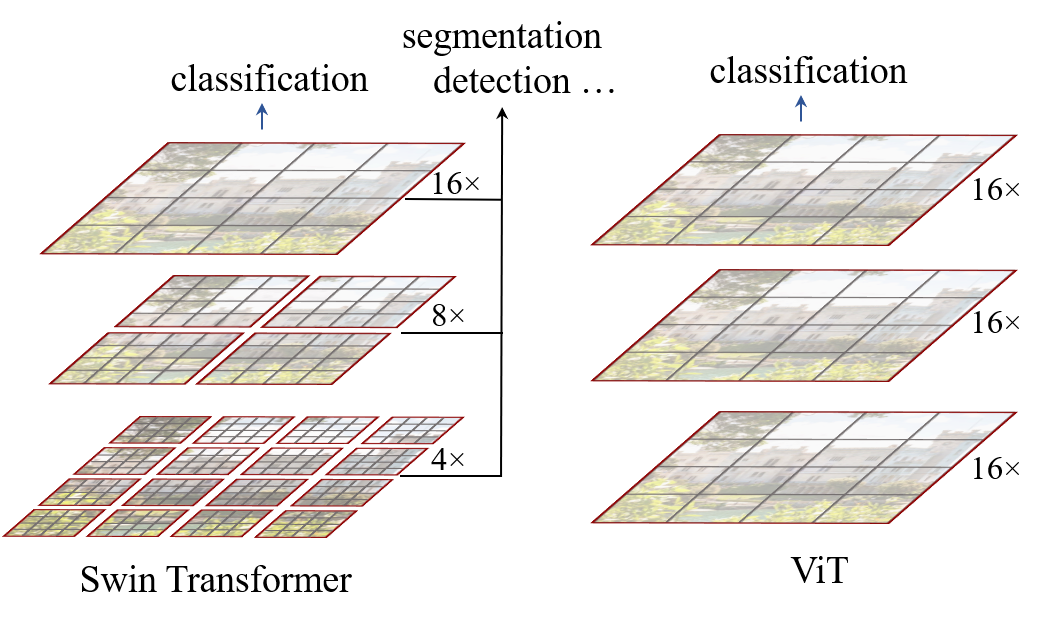
\includegraphics[width=\linewidth]{teaser11.png}
        \caption{ViT vs Swin transformer}
        \label{fig:swin-vit}
    \end{subfigure}\hfill
    \begin{subfigure}{0.45\textwidth}
        \centering
        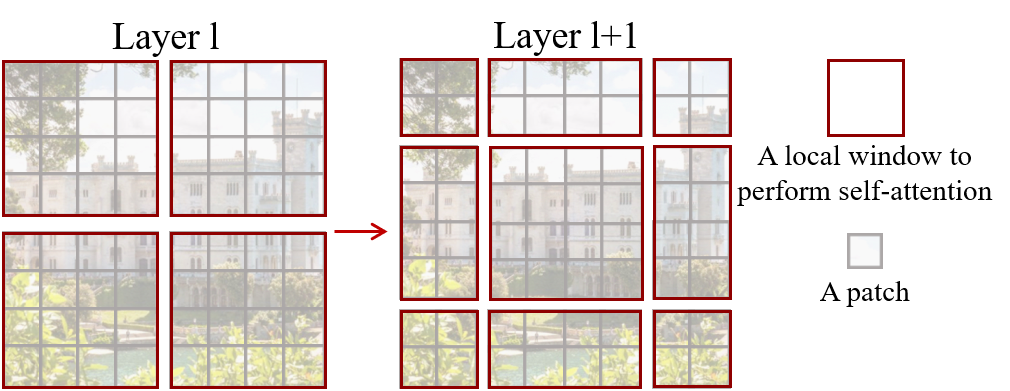
\includegraphics[width=\linewidth]{teaser_v4.png}
        \caption{The shifted window technique}
        \label{fig:shiftwindow}
    \end{subfigure}
    \caption{Characteristics of the Swin transformer\cite{DBLP:journals/corr/abs-2103-14030}}
    \label{fig:swintransform}
\end{figure}



\clearpage{}

\newcommand{\lt}{L\textsubscript{2}}

\section{Training Methodology}

\subsection{Loss function}
\label{loss_function_section}

The choice of loss function is crucial for the performance of our model.

In this assessment, we experimented with three different loss functions.

\begin{description}[style=nextline]
	\item[Categorical Cross-Entropy Loss] All pixels (except the ones marked as background) are equally weighted.
	\item[CCE loss ignoring background pixels] Pixels marked as background in the true mask are not counted for the loss.
	\item[Intersection over Union Loss] A differentiable version of IoU score, which should ideally work to maximise it.
	\item[Dice Loss] Categories that appear less often are weighted higher\cite{dice_loss}.
\end{description}

Using \textbf{Categorical Cross-Entropy} provided better results in the relevant metrics, including IoU score, when compared to both dice loss and IoU loss.

This surprising result, which can be seen in \cref{iou_vs_cce}, is likely due to the difference in depth of the loss functions.
Since it contradicts some existing literature\cite{dice_loss}, it warrants more exploration later.

Ignoring background pixels produces better metrics in IoU score than regular categorical cross-entropy.
However, a bad classifier might ``hallucinate'' bad pixels in areas of the background, and these false positives could cause bigger problem than unknown pixels despite not being part of the IoU Score.

The objective of this work is to produce a good mask for city scenes, so not ignoring pixels might be preferable despite the hit in metrics.
To produce a balanced approach, we will train the first two models (baseline and UNet) on regular categorical cross-entropy loss.

In our experiments the second enhanced model (Swin2-JNet) is considerably stronger and likely to have fewer false positives compared to the other models, so we will train it ignoring these background pixels to later compare it to the other models.

\begin{figure}[b]
	\centering
	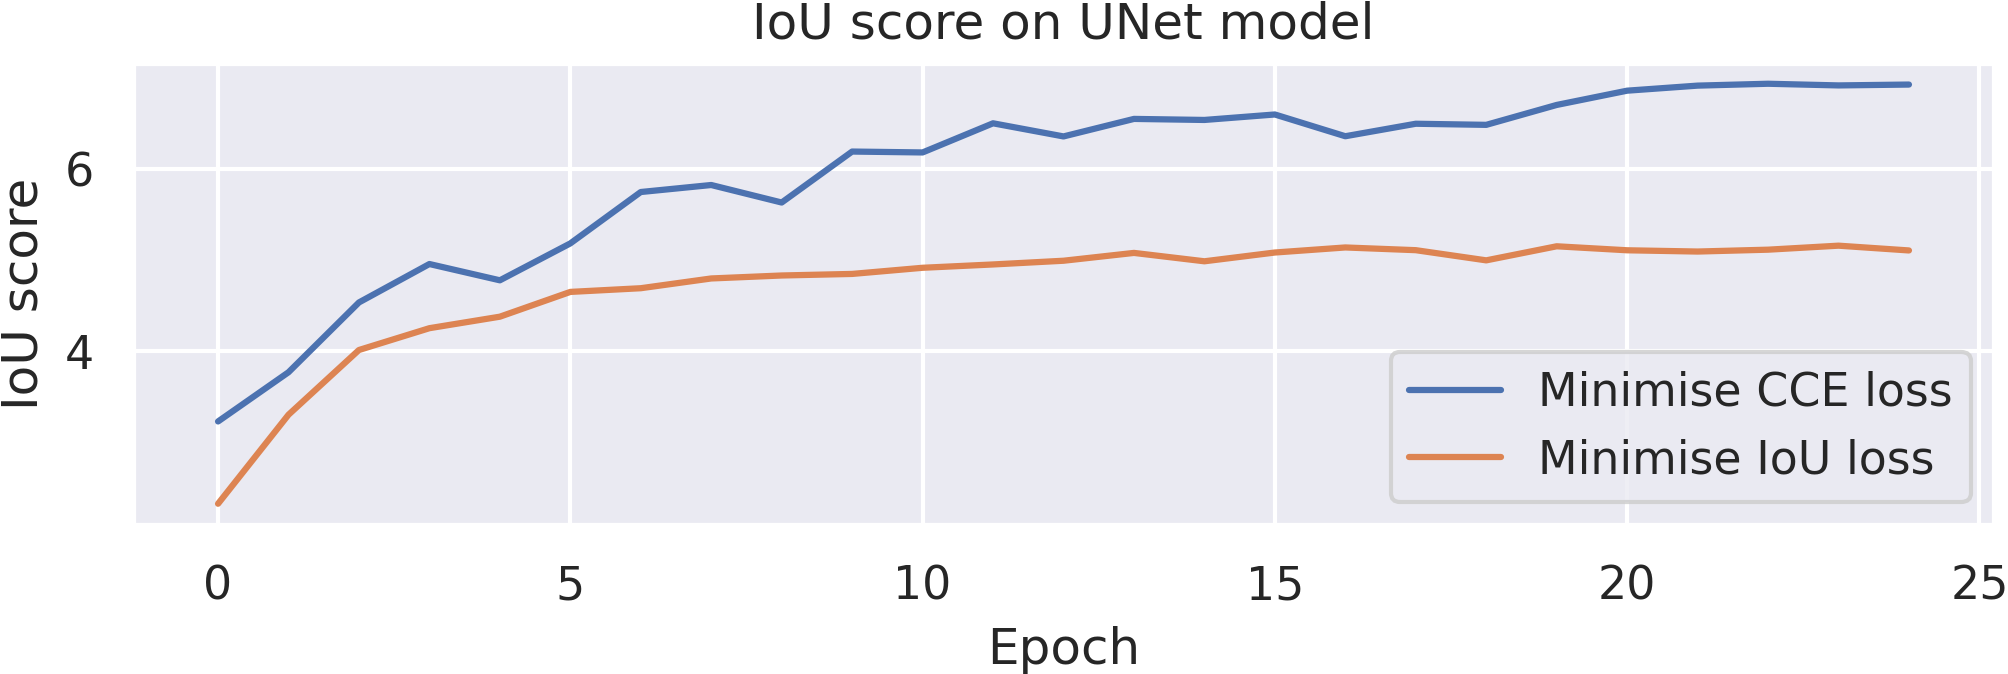
\includegraphics[width=.81\textwidth]{cce_vs_iou_loss.png}
	\caption{IoU score for an early model based on UNet that was trained to minimise both categorical cross-entropy and a related IoU loss depending on the epoch. Surprisingly, the one that optimises CCE has better results.}
	\label{iou_vs_cce}
\end{figure}

\subsection{Transforming and Enhancing Data}
% In our test runs, the images in the input data are resized to $768 \times 768$.
% This size presents a good balance between model performance and training speed: the final results of the models were almost identical to using the entire size of $2048 \times 1024$.
% Additionally, this new size makes it possible to use pretrained Swin2 in the entire data instead of having to separate the images of stretch it separately.

% The loss of the final mask is calculated on the small, resized image.
% When evaluating, the final mask is stretched to its original larger size.

% Additionally, we experimented with creating random transforms of the input data, including random flips and random crops.

We experimented with creating random transforms of the input data, including random flips and random crops.

In different experiments these transforms either replaced or augmented the original training data.
However, this is not present in the final models as their results weren't conclusive: since the original data is complete enough, adding these transforms only made the results on the validation set worse.

\subsection{Optimiser and Scheduler}

All mature models use the \textbf{AdamW} optimiser, which decouples weight decay from the optimisation process\cite{adamW}.
This model produced a more effective \lt{} regularisation than other similar classifiers, and generally better results than both the Adam and Adamax optimiser.

Initial experiments produced a clear overfit in most models after about 10 steps, which became noticeable after 20.
To prevent this overfitting, among many other solutions, we implemented a \textbf{Step Scheduler} which lowers the learning rate every 10 steps by a certain factor, $\gamma$.
This can be seen in \cref{gamma_vs_nogamma}.

\begin{figure}
	\centering
	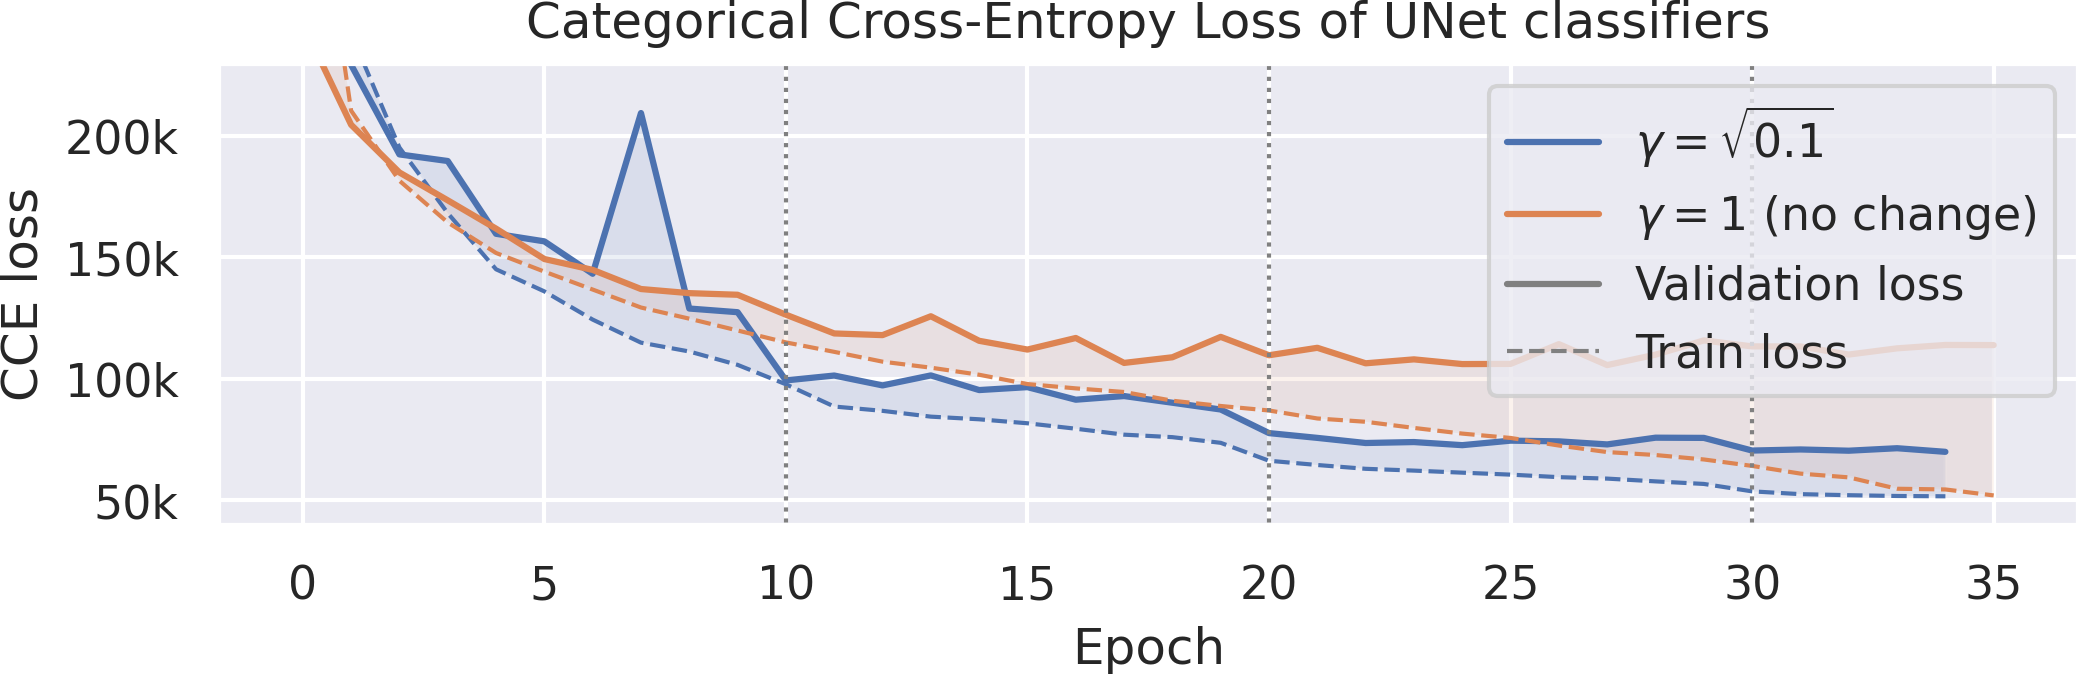
\includegraphics[width=.90\textwidth]{gamma_vs_nogamma.png}
	\caption{Differences between training and validation loss of a classifier that dynamically adjusts its learning rate every 10 steps and one that doesn't. While both classifiers overfit, the dynamic learning rate makes this process slower and the eventual validation loss reaches better values.}
	\label{gamma_vs_nogamma}
\end{figure}

The ideal value of $\gamma$ depends on other hyperparameters, and was thus found in a hyperparameter sweep in \cref{param_sweep_results}.

% \newpage{}
\subsection{Early Stopping}

Our input data is large and, even with many different kinds of regularisation, all models overfit after so many epochs.

To prevent this we only capture the classifier trained up to the epoch with the lowest validation loss.
This returns a model that's trained on subtle details that could help identify each pixel as a different class, but ignores noise on the training data that leads it to overfit.

\subsection{Halving Hyperparameter Sweep}
\label{param_sweep_section}
Some hyperparameters, such as the AdamW optimiser, were set early on as they produced consistently good results.

Others can change the loss function in unpredictable ways.
In order to test all of them, for the two enhanced models we run a hyperparameter sweep with the parameters in \cref{hyperparameter_list}.

\begin{table}[h]
	\centering
	\small
	\begin{tabular}{>{\bfseries}r | r r r}
		\toprule
		Hyperparameter & \multicolumn{3}{c}{Options} \\
		\midrule
		Initial Learning Rate & $10^{-3}$ & $10^{-4}$ & \\
		Learning Rate Decay $\gamma$ & 1 & $\sqrt{0.1}$ & $0.1$ \\
		\lt{} Weight Decay & $0$ & $10^{-4}$ & \\
		Dropout & 0 & $0.05$ & $0.1$ \\
		\bottomrule
	\end{tabular}
	\caption{Parameter list for hyperparameter sweep}
	\label{hyperparameter_list}
\end{table}

The entire dataset of 2975 images is very large, and making this 36-parameter sweep cost-prohibitive.

To run a parameter sweep on all possible combinations of hyperparameters, we instead run a \textbf{Halving Parameter Sweep}\cite{halving_param_sweep}.
\begin{enumerate}
	\item Train classifiers for 20 epochs using a randomly sampled subset of the data for each combination of hyperparameters.
	\item Split the results in two. Discard the half with the highest validation loss, and keep the half with the lower loss.
	\item Double the amount of data used for the training, and repeat.
\end{enumerate}

This method makes it possible to discard the least promising results early on, while focusing most time and computing power on the most promising candidates.
The top 2 candidates are trained using the whole dataset.

The results can be found in \cref{param_sweep}, with the best parameters in \cref{param_sweep_results}.

\begin{table}[h]
	\centering
	\small
	\begin{tabular}{>{\bfseries}r | c c c c | r c c}
		\toprule
		Model & LR & $\gamma$ & \lt{} & Dropout & Val Loss & IoU & \iiouc{} \\
		\midrule
		UNet & $10^{-3}$ & $\sqrt{0.1}$ & $0$ & & \num{221343} & 17.56 & 20.30 \\
		Swin2-J & $10^{-3}$ & 1 & $10^{-4}$ & $0.05$ & \num{78946} & 25.47 & 27.60 \\
		\bottomrule
	\end{tabular}
	\caption{Parameters with best validation loss in the last round of the halving hyperparameter sweep.}
	\label{param_sweep_results}
\end{table}

The scores of this parameter sweep will likely be lower than the final scores of the models since even at the last stage they are training with less data.

However, we can be relatively certain that the \emph{order} of the results of each step is roughly correct.

\newpage{}
In addition to the best hyperparameters for our models, this parameter sweep gives some interesting information about the models.
\begin{enumerate}
	\item In both cases, runs with $\text{LR} = 10^{-3}$ beat the ones with $\text{LR} = 10^{-4}$. The second initial learning rate is likely too small.
		\emph{All} of the models that lost the first round have $\text{LR} = 10^{-4}$.
	\item In the UNet model, both a variable learning rate and a nonzero \lt{} weight decay are good predictors for validation loss.
		This is not true in the Swin2-JNet model, where models with positive weight decay and no variable learning rate have a consistently better validation loss than ones with variable learning rate.
		This second case is likely due to dropout: the winner models have positive dropout (not shown in the scatterplot due to lack of dimensionality), which prevents overfitting better than a variable learning rate.
	\item In a similar way, the strong regularisation provided by dropout makes the case of $\gamma = 1$ the best for the Swin2-JNet model.
\end{enumerate}

\vfill{}

\begin{figure}[h]
	\begin{subfigure}[t]{.35\textwidth}
		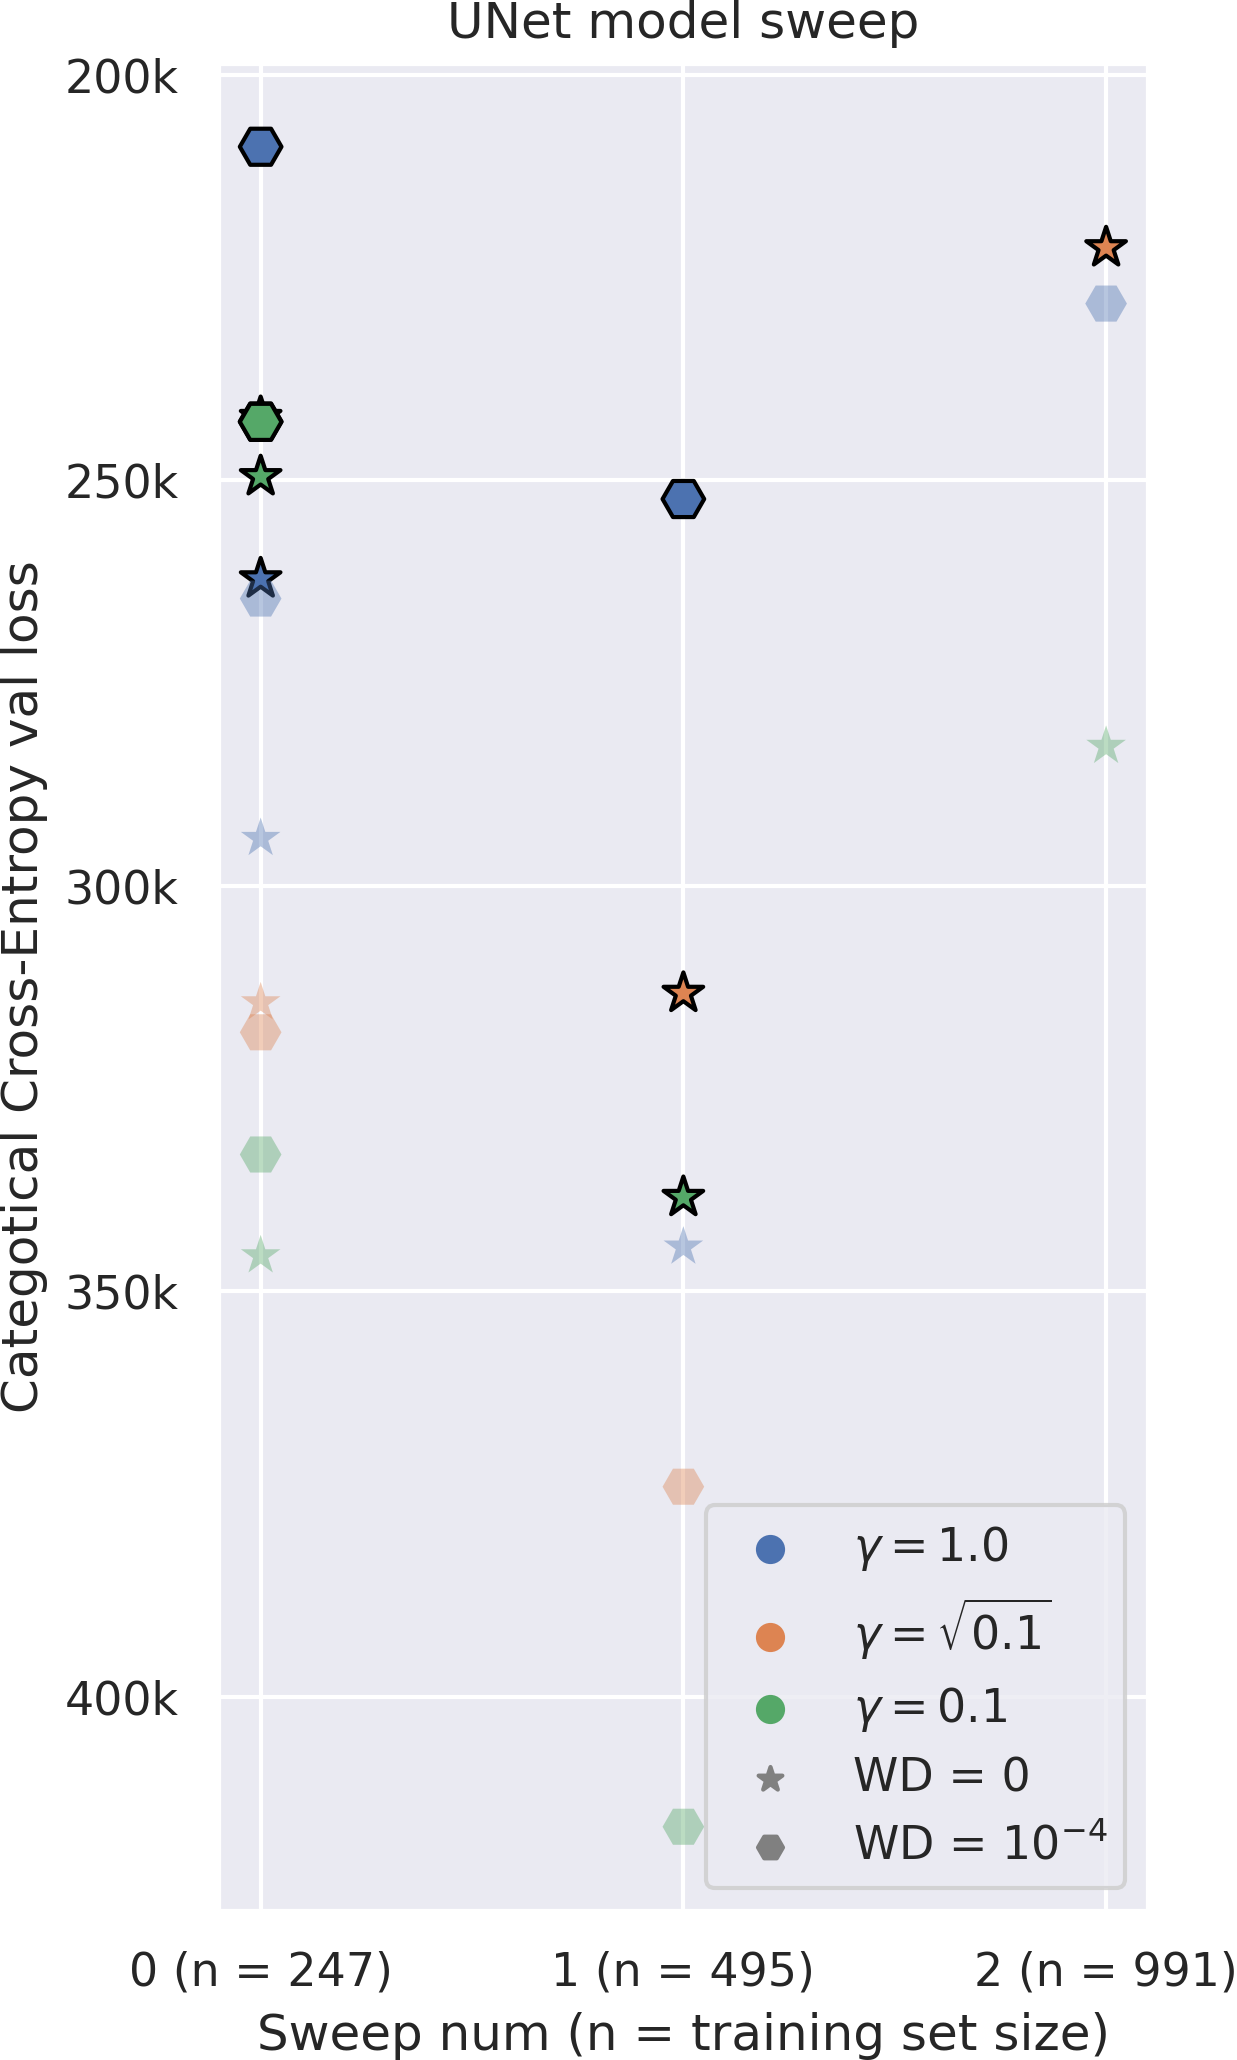
\includegraphics[height=300pt]{unet_sweep.png}
		\caption{Halving hyperparameter sweep for UNet model.}
		\label{unet_param_sweep}
	\end{subfigure} \hfill{}
	\begin{subfigure}[t]{.65\textwidth}
		\hfill{}
		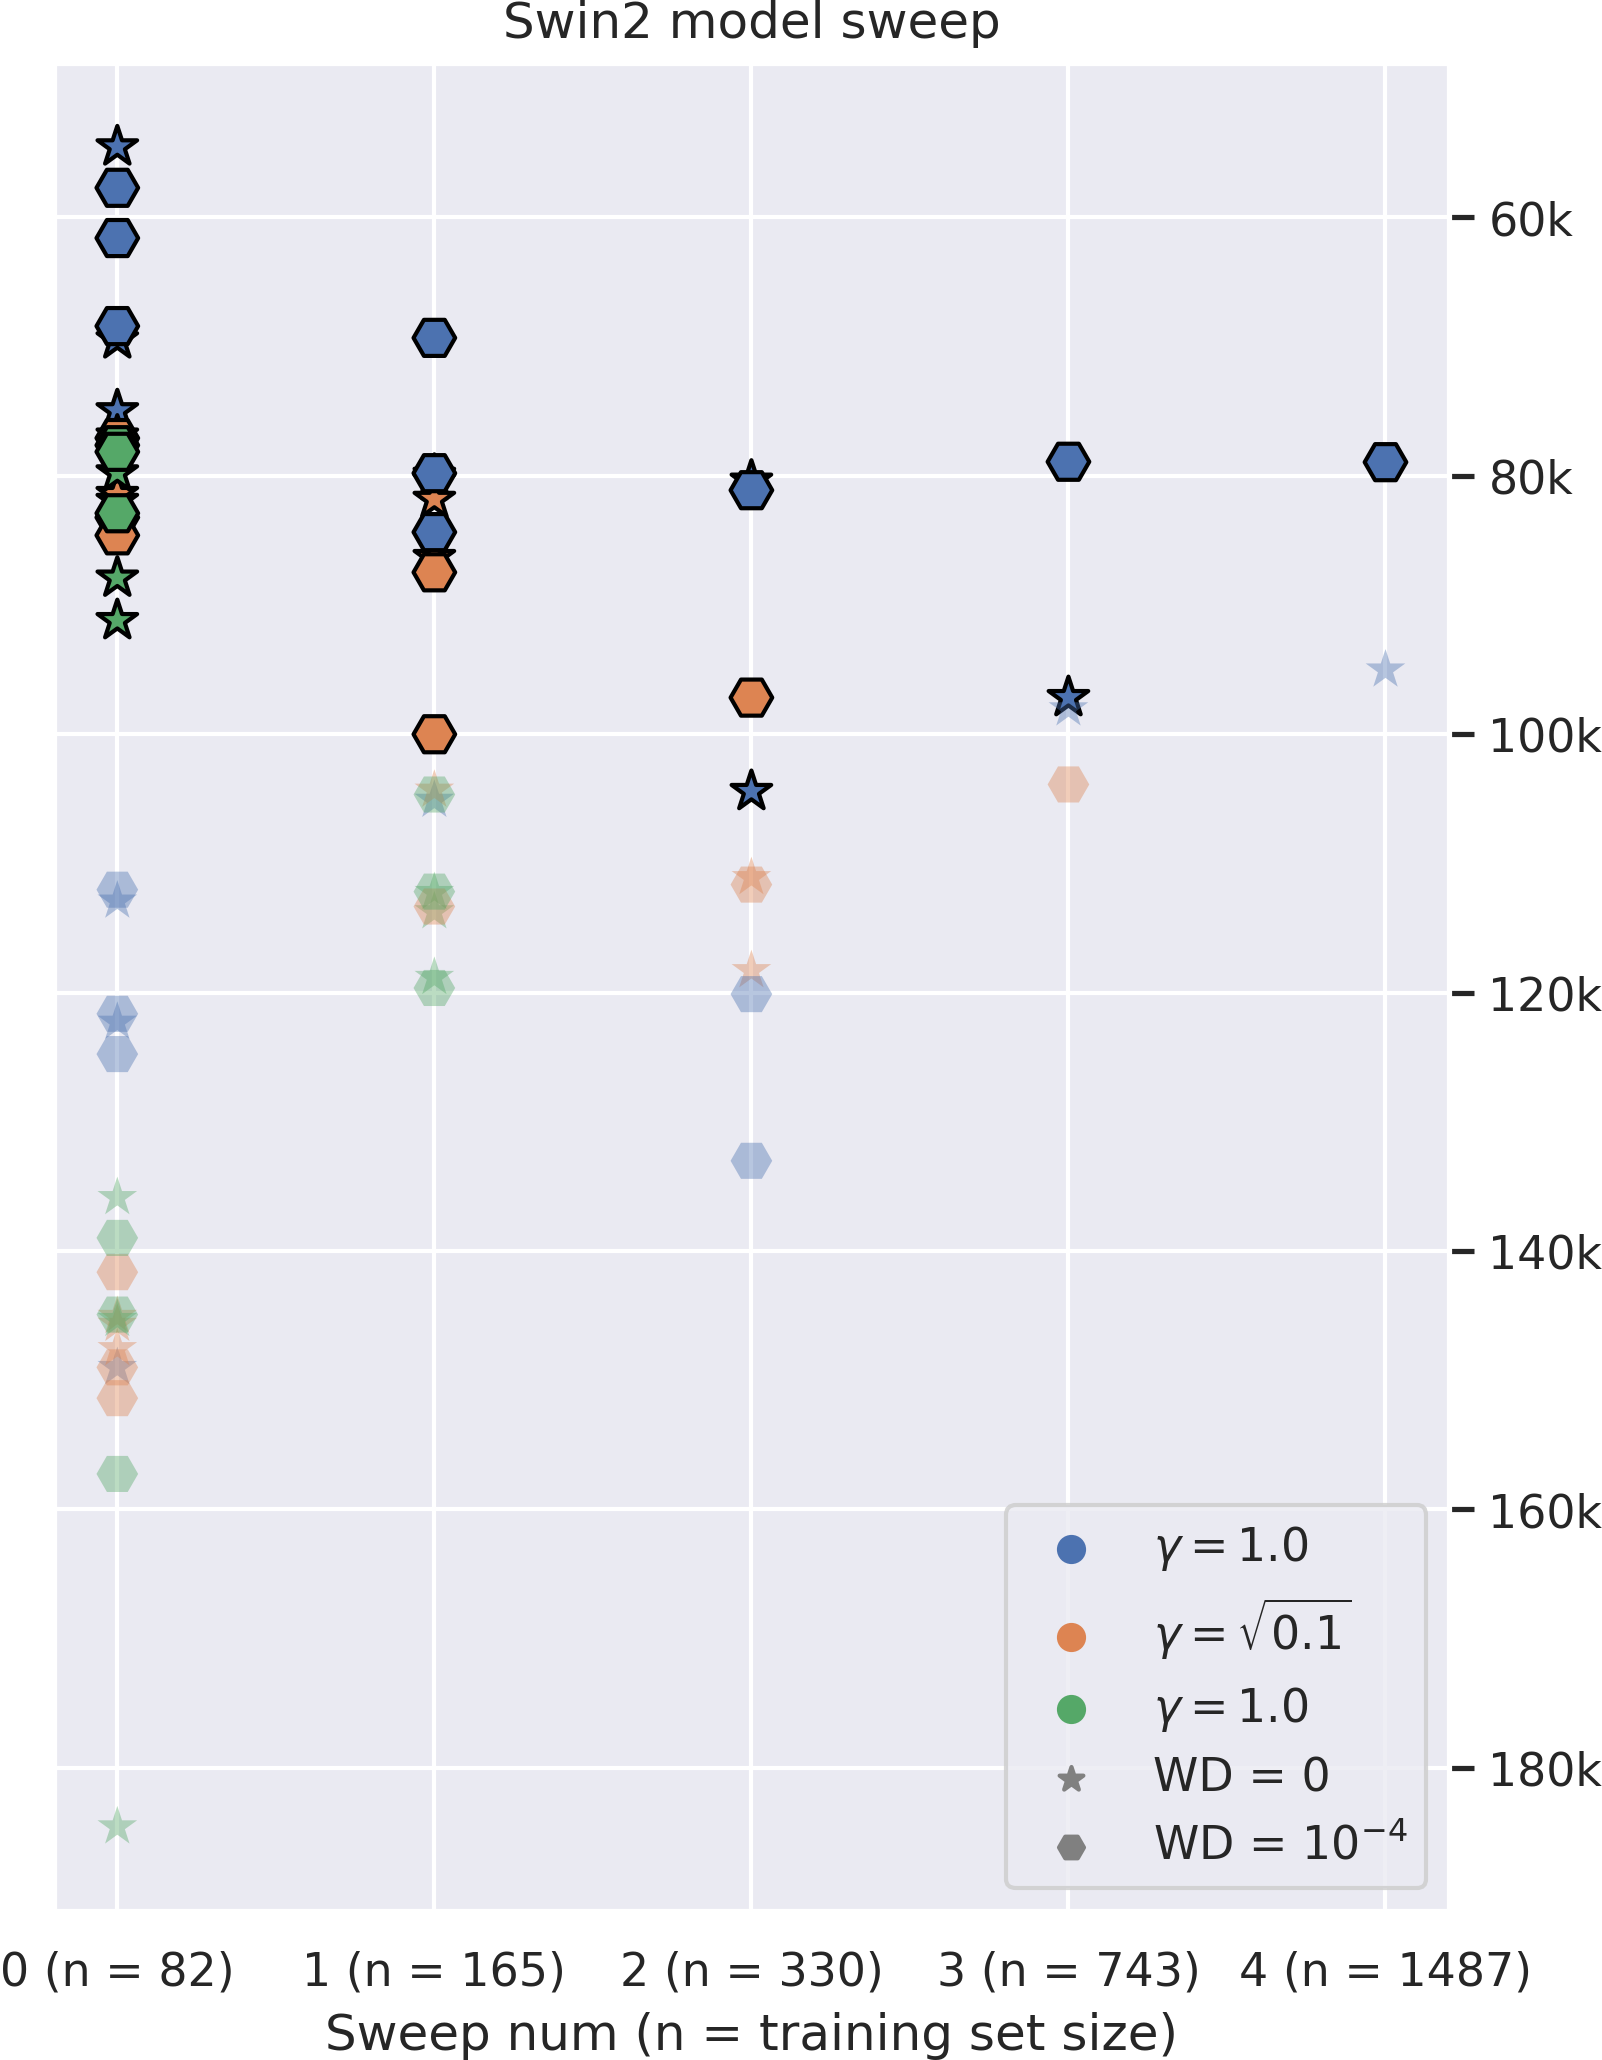
\includegraphics[height=300pt]{swin2_sweep.png}
		\caption{Halving hyperparameter sweep for Swin2-JNet model.}
		\label{swin2_param_sweep}
	\end{subfigure}
	\caption{Results of the halving hyperparameter sweep for both enhanced models. Transparent points are ones that are over the 50\% of CCE loss in each sweep, which didn't make it to the next one. Validation loss is wildly different between sweeps since each one uses a different subset of training and validation loss: the ordering matters, but the values themselves are meaningless.}
	\label{param_sweep}
\end{figure}



\clearpage{}

\section{Results}


\clearpage{}

\section{Conclusions and Reflections}

This project was a long and thorough work over the CityScapes dataset.
We changed many metrics, objectives, and models throughout its lifetime, learned from those changes, and changed everything again.

From the models we tried, Swin2-JNet is the clear winner.
Not only it has the highest IoU and \iiouc{} scores of the dataset by a little, as shown in \cref{which_one_wins}, but when testing these models on real-world data in \hyperref[hackneyscapes]{Appendix A} the results are considerably nicer.

Why is this model better than UNet, which has an equivalent size?
We propose several reasons.
\begin{enumerate}[topsep=0pt]
	\item The attention in the Swin2 transformers provide a significative improvement to small details, such as people in the background.
	\item Using transfer learning from a pre-trained means that a lot of basic data, such as lines of objects, are already learned.
		\begin{enumerate}
			\item Moreover, the use of skip connections with the data from a feature pyramid allows the classifier to learn from several resolutions of this feature.
		\end{enumerate}
	\item Not learning on ``background'' pixels (which were mostly arbitrary) saved some capacity on the model to learn extra details, and helped it generalise more.
		\begin{enumerate}
			\item Note that earlier, smaller experiments with other models resulted in a lot of incorrect positives on these background pixels.
				This property was a last-minute addition, and it might make sense to review the previous experiments.
		\end{enumerate}
	\item Effective use of Dropout prevented bad overfitting.
		It's easy to compare \cref{unet_model_loss} with \cref{swin2_model_loss} and realise that, while early stopping prevented the model from learning many incorrect details, the UNet model is still not able to learn some correct ones due to how badly it overfits.
\end{enumerate}

The most effective part of this project was its infrastructure: having a pre-set files to allow us to train models quickly and easily (along with the help of Wandb) allowed us to iterate quickly and try a lot of experiments.

Additionally, having two canonical metrics we do not train in (IoU and \iiouc{} scores) allowed us to compare different models easily.

Most importantly, the halving parameter sweep in \cref{param_sweep_section} allowed us to find and compare dozens of different hyperparameter combinations in a reasonable amount of time.

The CityScapes dataset did not provide a test set, as it's secret to be submitted\cite{cityscapes_benchmark}.
In the near future we plan to train our Swin2-JNet model classifier in both the training and validation data and submit it to the Benchmark suite.
If our calculations in the validation set are roughly correct, we should be roughly in the best two thirds of \href{https://www.cityscapes-dataset.com/benchmarks/#pixel-level-results}{the CityScapes Benchmark Competition}, despite not even using the fine dataset.

The objective of this project was not to win a competition, which is why it's important to be wary of overfocusing on maximising metrics.
While the IoU score could might have been higher, the results in our own subjective test set of \hyperref[hackneyscapes]{HackneyScapes} speak for themselves.


\clearpage{}

	section{Reflections}


\clearpage{}

\bibliography{convolutional_assessment}

\end{document}
